<<<<<<< HEAD
\begin{name}
	{ÔN TẬP KTTX 2}
	{TOÁN 10}
	{LỚP TOÁN THẦY PHÁT}
	{Thời gian: 90 phút - Không kể thời gian phát đề}
\end{name}
\TN
\setcounter{ex}{0}\setcounter{ex}{0}
\Opensolutionfile{ans}[ans/ans-KT-301]
=======
\def\tenchude{ÔN TẬP KTTX 2}
\begin{name}
	{\tenchude}
	{TOÁN 10}
	{LỚP TOÁN THẦY PHÁT}
	{Thời gian không chờ đợi ai, đừng lãng phí!}
\end{name}

\setcounter{ex}{0}\setcounter{ex}{0}
\Opensolutionfile{ans}[ans/ans-KT-301]

>>>>>>> fb6a4a45986863e8605634e31e689e31425c42cc
\begin{ex}
	Giá trị lượng giác nào sau đây là số dương?
	\choice
	{\True $\sin 120^\circ$}
	{$\cos 137^\circ$}
	{$\tan 160^\circ$}
	{$\cot 160^\circ$}
	\loigiai{
		Ta có $90^\circ<120^\circ<180^\circ$ nên $\sin 120^\circ>0$.\\
		Do $90^\circ<137^\circ<180^\circ$ nên $\cos 137^\circ<0$.\\
		Ngoài ra, $90^\circ<160^\circ<180^\circ$ nên $\tan 160^\circ<0$ và $\cot 160^\circ<0$.
	}
\end{ex}

\begin{ex}
	Cho $\sin\alpha=\dfrac{4}{5}$, $\left(90^\circ<\alpha <180^\circ\right)$. Tính $\cos\alpha $.
	\choice
	{$\cos\alpha=-\dfrac{4}{5}$}
	{\True $\cos\alpha=-\dfrac{3}{5}$}
	{$\cos\alpha=\dfrac{5}{3}$}
	{$\cos\alpha=\dfrac{3}{5}$}
	\loigiai{
		Ta có $\sin^2\alpha+\cos^2\alpha=1$ $\Leftrightarrow \cos^2\alpha=1-\sin^2\alpha=1-\dfrac{16}{25}=\dfrac{9}{25}\Rightarrow\cos\alpha=\pm\dfrac{3}{5}$.\\
		Mặt khác $90^\circ<\alpha<180^\circ$ nên $\cos\alpha=-\dfrac{3}{5}$.}
\end{ex}

\begin{ex}
	Cho $x\in\left(0^\circ;90^\circ\right)$. Phát biểu nào sau đây là đúng?
	\choice
	{\True $\sin x>0$}
	{$\cos x>0$}
	{$\tan x>0$}
	{$\cot x>0$}
	\loigiai{
		Khi $x\in\left(\dfrac{5\pi}{2};3\pi\right)$ thì $\heva{&\sin x>0\\&\cos x<0\\&\tan x<0\\&\cot x<0.}$ }
<<<<<<< HEAD
=======
\end{ex}

\begin{ex}
	Giá trị $\cos 45^\circ+\sin 45^\circ$ bằng bao nhiêu?
	\choice
	{$1$}
	{\True $\sqrt{2}$}
	{$\sqrt{3}$}
	{$0$}
	\loigiai
	{Bằng cách tra bảng giá trị lượng giác của các góc đặc biệt hay dùng MTCT ta được $\heva{& \cos 45^\circ=\dfrac{\sqrt{2}}{2} \\
				& \sin 45^\circ=\dfrac{\sqrt{2}}{2} \\
			}$\\
		$\Rightarrow \cos 45^\circ+\sin 45^\circ=\sqrt{2}$.}
\end{ex}
\begin{ex}
	Giá trị của $\cot18^\circ$ là
	\choice
	{$1$}
	{$-1$}
	{$0$}
	{\True $\sqrt{5+2\sqrt{5}}$}
	\loigiai{
		Ta có $\cot18^\circ=\sqrt{5+2\sqrt{5}}$.
	}
>>>>>>> fb6a4a45986863e8605634e31e689e31425c42cc
\end{ex}
\begin{ex}
	Trên nửa đường tròn đơn vị cho góc $\alpha$ sao cho $\sin\alpha=\dfrac{2}{3}$ và $\cos\alpha<0$. Tính $\tan\alpha$.
	\choice
	{\True $-\dfrac{2\sqrt{5}}{5}$}
	{$\dfrac{2\sqrt{5}}{5}$}
	{$-\dfrac{2}{5}$}
	{$1$}
	\loigiai{
		Ta có $\cos\alpha=-\sqrt{1-\sin^2\alpha}=-\dfrac{\sqrt{5}}{3}$ suy ra $\tan\alpha=-\dfrac{2\sqrt{5}}{5}$.
	}
\end{ex}
\begin{ex}
	Cho $\sin x+\cos x=\dfrac{1}{2}$ và $0<x<90^\circ$. Tính giá trị của $\sin x$
	\choice
	{$\sin x=\dfrac{1+\sqrt{7}}{-6}$}
	{$\sin x=\dfrac{1-\sqrt{7}}{6}$}
	{\True $\sin x=\dfrac{1+\sqrt{7}}{4}$}
	{$\sin x=\dfrac{1-\sqrt{7}}{4}$}
	\loigiai{
		Vì $0<x<90^\circ$ nên $\sin x>0$. Ta có
		\begin{eqnarray*}
			\sin^2x+\cos^2x=1 &\Leftrightarrow&\sin^2x+\left( \dfrac{1}{2}-\sin x\right)^2 =1\\
			&\Leftrightarrow& 2\sin^2x-\sin x-\dfrac{3}{4}=0\\
			&\Leftrightarrow& \hoac{&\sin x=\dfrac{1+\sqrt{7}}{4}\\&\sin x=\dfrac{1-\sqrt{7}}{4} \text{ (loại).}}
		\end{eqnarray*}
	}
\end{ex}
\begin{ex}
	Chọn phát biểu đúng trong các phát biểu sau?
	\choice
	{$\sin 156^\circ\cdot\cos70^\circ<0$}
	{$\tan 137^\circ\cdot\tan 156^\circ<0$}
	{\True $\tan150^\circ\cdot\cot85^\circ<0$}
	{$\sin 110^\circ\cdot\cos 110^\circ>0$}
	\loigiai{
		\begin{enumerate}
			\item Do $\heva{&\sin156^\circ>0\\&\cos70^\circ>0}$ nên $\sin 156^\circ\cdot \cos(-70^\circ)>0$.
			\item Do $\heva{&\tan 137^\circ<0\\&\tan 156^{\circ}<0}$ nên $\tan 137^\circ\cdot \tan 156^\circ>0$.
			\item Do $\heva{&\tan 150^\circ>0\\&\cot 85^\circ>0}$ nên $\tan 150^\circ\cdot\cot 85^\circ<0$.
			\item Do $\heva{&\sin 110^\circ>0\\&\cos 110^\circ<0}$ nên $\sin 110^\circ\cdot\cos 110^\circ<0$.
		\end{enumerate}
	}
\end{ex}
\begin{ex}
	Phát biểu nào sau đây là đúng?
	\choice
	{$\sqrt{1-\sin^2 140^\circ}=\cos 140^\circ$}
	{\True $\sqrt{1-\cos^2 140^\circ}=\sin 140^\circ$}
	{$\sqrt{\dfrac{1}{\cos^2 140^\circ}-1}=\tan 140^\circ$}
	{$\dfrac{1}{\sqrt{\tan^2 140^\circ+1}}=\cos 140^\circ$}
	\loigiai{
		Do $140^\circ\in\left(90^\circ;180^\circ\right)$ nên $\heva{&\sin 140^\circ>0\\&\cos 140^\circ<0\\&\tan 140^\circ<0\\&\cot 140^\circ<0}$ nên $\heva{&\sqrt{1-\sin^2 140^\circ}=-\cos 140^\circ\\ &\sqrt{1-\cos^2 140^\circ}=\sin 140^\circ\\& \sqrt{\dfrac{1}{\cos^2 140^\circ}-1}=-\tan 140^\circ\\ &\dfrac{1}{\sqrt{\tan^2 140^\circ+1}}=-\cos 140^\circ.}$
	}
\end{ex}
\begin{ex}
	Tìm mệnh đề \textbf{sai} trong các mệnh đề sau
	\choice
	{$\cos 0^\circ=1$}
	{$\sin 0^\circ=0$}
	{\True $\cos 120^\circ=\dfrac{2}{\sqrt{2}}$}
	{$\sin 120^\circ=\dfrac{\sqrt{3}}{2}$}
	\loigiai{
		Mệnh đề sai là $\cos 120^\circ=\dfrac{2}{\sqrt{2}}$ vì $\cos 120^\circ=-\cos 60^\circ=\dfrac{\sqrt{3}}{2}$.
	}
\end{ex}
\begin{ex}
	Cho $\alpha$ là góc tù. Mệnh đề nào đúng trong các mệnh đề sau?
	\choice
	{$\sin\alpha<0$}
	{$\cos\alpha>0$}
	{\True $\tan\alpha<0$}
	{$\cot\alpha>0$}
	\loigiai{
		Vì $\alpha$ là góc tù nên $\tan\alpha<0$.
	}
\end{ex}
\begin{ex}
	Trong các mệnh đề sau, mệnh đề nào \textbf{sai}?
	\choice
	{$\cos 45^\circ=\sin 45^\circ$}
	{$\cos 45^\circ=\sin 135^\circ$}
	{$\cos 30^\circ=\sin 120^\circ$}
	{\True $\sin 60^\circ=\cos 120^\circ$}
	\loigiai{
		Ta có $\sin 60^\circ=\dfrac{\sqrt{3}}{2}$ và $\cos 120^\circ=-\cos 60^\circ=-\dfrac{1}{2}$.\\
		Do đó mệnh đề sai là $\sin 60^\circ=\cos 120^\circ$.
	}
\end{ex}
\begin{ex}
	Cho hai góc nhọn $\alpha$ và $\beta$ với $\alpha<\beta$. Tìm mệnh đề \textbf{sai}.
	\choice
	{$\sin\alpha<\sin\beta$}
	{\True $\cos\alpha<\cos\beta$}
	{$\cos\alpha=\sin\beta\Leftrightarrow \alpha+\beta=90^\circ$}
	{$\tan\alpha+\tan\beta>0$}
	\loigiai{
		Ta có mệnh đề \textbf{sai} là $\cos\alpha<\cos\beta$.
	}
\end{ex}
\begin{ex}
	Cho $0^{\circ}\leq\alpha\leq 180^{\circ}$. Khẳng định nào sau đây là đúng?
	\choice
	{\True $\sin\alpha=\sin(180^{\circ}-\alpha)$}
	{$\cos\alpha=\cos(180^{\circ}-\alpha)$}
	{$\tan\alpha=\tan(180^{\circ}-\alpha)$}
	{$\cot\alpha=\cot(180^{\circ}-\alpha)$}
	\loigiai{
		Khẳng định đúng là $\sin\alpha=\sin(180^{\circ}-\alpha)$.
	}
\end{ex}
\begin{ex}
	\immini{Trên nửa đường tròn đơn vị, vị trí nào trong các vị trí dưới đây xác định điểm $M$ sao cho $\tan\widehat{xOM}=1$.
		\choice
		{\True Vị trí $(1)$}
		{Vị trí $(2)$}
		{Vị trí $(3)$}
		{Vị trí $(4)$}
	}
	{
		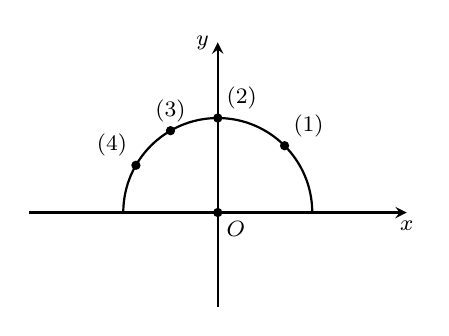
\begin{tikzpicture}[>=stealth,x=1.0cm,y=1.0cm,thick,scale=1.2]
			\begin{footnotesize}
				\draw[->] (-2,0) -- (2,0) node[below] {$x$};
				\draw[->] (0,-1) -- (0,1.8) node[left] {$y$};
				\coordinate (O) at (0,0);
				\fill[black] (0,0) circle[radius=1.4pt] node[below right]{\footnotesize $O$};
				\coordinate (M) at (0.7071,0.7071);
				\fill[black] (0.7071,0.7071) circle[radius=1.4pt] node[above right]{\footnotesize $(1)$};
				\draw (1,0) arc (0:180:1);
				\coordinate (P) at (-0.866,0.5);
				\fill[black] (-0.866,0.5) circle[radius=1.4pt] node[above left]{\footnotesize $(4)$};
				\coordinate (N) at (-0.5,0.866);
				\fill[black] (-0.5,0.866) circle[radius=1.4pt] node[above ]{\footnotesize $(3)$};
				\coordinate (Q) at (0,1);
				\fill[black] (0,1) circle[radius=1.4pt] node[above right]{\footnotesize $(2)$};

			\end{footnotesize}
		\end{tikzpicture}
	}
	\loigiai{
		Ở vị trí $1$ ta có $\sin\widehat{xOM}=\cos\widehat{xOM}$ nên $\tan\widehat{xOM}=1$.
	}
<<<<<<< HEAD
=======
\end{ex}
\begin{ex}
	Cho hai góc $\alpha$ và $\beta$ với $\alpha+\beta =180^\circ$. Tính giá trị của biểu thức $P=\cos\alpha\cos\beta -\sin\beta\sin\alpha$.
	\choice
	{$P=0$}
	{$P=1$}
	{\True $P=-1$}
	{$P=2$}
	\loigiai
	{Hai góc $\alpha$ và $\beta$ bù nhau nên $\sin\alpha =\sin\beta$; $\cos\alpha =-\cos\beta$.\\
		Do đó $P=\cos\alpha\cos\beta -\sin\beta\sin\alpha =-\cos^2\alpha -\sin^2\alpha =-(\sin^2\alpha +\cos^2\alpha)=-1$.}
>>>>>>> fb6a4a45986863e8605634e31e689e31425c42cc
\end{ex}

\begin{ex}
	Khẳng định nào sau đây \textbf{sai}?
	\choice
	{\True $\cos 75^\circ >\cos 50^\circ $}
	{$\sin 80^\circ >\sin 50^\circ $}
	{$\tan 45^\circ <\tan 60^\circ $}
	{$\cos 30^\circ =\sin 60^\circ $}
	\loigiai
	{Trong khoảng từ $0^\circ$ đến $90^\circ$, khi giá trị của góc tăng thì giá trị $\cos$ tương ứng của góc đó giảm.}
\end{ex}
<<<<<<< HEAD

=======
\begin{ex}
	Cho tam giác $MNP$ không vuông có diện tích là $S$, $p$ là nửa chu vi, $r$ là bán kính đường tròn nội tiếp và $R$ là bán kính đường tròn ngoại tiếp. Khẳng định nào sau đây là khẳng định \textbf{sai}?
	\choice
	{\True $S=\dfrac{1}{2}MN\cdot MP$}
	{$S=p\cdot r$}
	{$S=\dfrac{MN\cdot MP\cdot NP}{4R}$}
	{$S=\dfrac{1}{2}NM\cdot NP\cdot\sin{N}$}
	\loigiai{
		Khẳng định \textbf{sai} là $S=\dfrac{1}{2}MN\cdot MP$.
	}
\end{ex}
>>>>>>> fb6a4a45986863e8605634e31e689e31425c42cc
\begin{ex}
	Tam giác $ABC$ vuông tại $A$ và có $AB=AC=a$. Tính độ dài đường trung tuyến $BM$ của tam giác đã cho.
	\choice
	{\True $BM=\dfrac{\sqrt{5}}{2}a$}
	{$BM=1{,}5a$}
	{$BM=\sqrt{2}a$}
	{$BM=\sqrt{3}a$}
	\loigiai{
		\immini{
			$M$ là trung điểm của $AC\Rightarrow AM=\dfrac{AC}{2}=\dfrac{a}{2}$.\\
			Xét tam giác $BAM$ vuông tại $A$, ta có\\
			$BM=\sqrt{AB^2+AM^2}=\sqrt{a^2+\dfrac{a^2}{4}}=\dfrac{a\sqrt{5}}{2}$.}
		{
			\begin{tikzpicture}[scale=1,font=\footnotesize,line join=round, line cap=round,>=stealth]
				\tkzDefPoints{0/0/A,0/3/B,4/0/C}
				\tkzDefMidPoint(A,C) \tkzGetPoint{M}
				\tkzDrawPoints[fill=black](A,B,C,M)
				\tkzDrawPolygon(A,B,C)
				\tkzDrawSegments(B,M)
				\tkzLabelPoints[above](B)
				\tkzLabelPoints[below](M,C,A)
				\tkzMarkRightAngles[size=0.2](C,A,B)
			\end{tikzpicture}
		}
	}
\end{ex}
\begin{ex}
	Cho tam giác $ABC$ có $3$ cạnh là $4$ cm, $8$ cm và $6$ cm. Tính diện tích tam giác $ABC$.
	\choice
	{$3\sqrt{5}$ cm $^2$}
	{$2\sqrt{10}$ cm $^2$}
	{$2\sqrt{15}$ cm $^2$}
	{\True $3\sqrt{15}$ cm $^2$}
	\loigiai{
		Ta có nửa chu vi $\triangle ABC$ là $p=\dfrac{4+8+6}{2}=9$ cm.\\
<<<<<<< HEAD
		Diện tích $\triangle ABC$ là $S_{\triangle ABC}=\sqrt{9(9-4)(9-6)(9-8)}=3\sqrt{15}$ cm $^2$.
=======
		Diện tích $\triangle ABC$ là $S_{\triangle ABC}=\sqrt{9(9-4)(9-6)(9-8)}=3\sqrt{15}$ cm $^2$.\\
		Suy ra bán kính $r$ của đường tròn nội tiếp tam giác $ABC$ là $r=\dfrac{S_{\triangle ABC}}{p}=\dfrac{3\sqrt{15}}{9}=\dfrac{\sqrt{15}}{3}$ cm.
>>>>>>> fb6a4a45986863e8605634e31e689e31425c42cc
	}
\end{ex}
\begin{ex}
	Cho tam giác $ABC$ có $\widehat{A}=30^\circ$, $\widehat{B}=45^\circ$ và $AC=10\sqrt{2}$. Độ dài cạnh $BC$ là
	\choice
	{\True $10$}
	{$5\sqrt{2}$}
	{$\dfrac{5}{\sqrt{2}}$}
	{$5$}
	\loigiai{
		Ta có $\dfrac{AC}{\sin B}=\dfrac{BC}{\sin A}\Rightarrow BC=\dfrac{AC\cdot\sin A}{\sin B}=\dfrac{10\sqrt{2}\cdot\sin 30^\circ}{\sin 45^\circ}=10$.
	}
\end{ex}
\begin{ex}
	Cho tam giác $ABC$ có nửa chu vi $p=\dfrac{a+b+c}{2}$. Khẳng định nào sau đây là đúng?
	\choice
	{$S=\sqrt{pabc}$}
	{\True $S=\dfrac12 ab \sin C$}
	{$a^2=b^2+c^2+2bc\cos A$}
	{$S=p(a+b+c)$}
	\loigiai{
		Dựa vào công thức diện tích tam giác ta có $S=\dfrac12 ab \sin C$.
	}
\end{ex}
\begin{ex}
	Tính diện tích của tam giác $ABC$ có $b=2$, $\widehat{B}=30^\circ$, $\widehat{C}=45^\circ$.
	\choice
	{$2+2\sqrt{3}$}
	{$1$}
	{$\sqrt{3}$}
	{\True $1+\sqrt{3}$}
	\loigiai{
		Ta có: $\dfrac{b}{\sin B}=\dfrac{c}{\sin C}$. \\
		Suy ra $c=\dfrac{b\cdot \sin C}{\sin B}=\dfrac{2\cdot \sin 45^\circ}{\sin 30^\circ}=2\sqrt{2}$.\\
		Ta có $\widehat{A}=180^\circ-\widehat{B}-\widehat{C}=180^\circ-30^\circ-45^\circ=105^\circ$.\\
		Ta có $S=\dfrac{1}{2}bc\sin A=\dfrac{1}{2}\cdot 2\cdot 2\sqrt{2}\cdot \sin 105^\circ=1+\sqrt{3}$.
	}
\end{ex}
\begin{ex}
	Trong tam giác $ABC$ có góc $\widehat{A}=60^{\circ}$, $AC=10$, $AB=6$. Khi đó, độ dài cạnh $BC$ là
	\choice
	{\True $2\sqrt{19}$}
	{$76$}
	{$14$}
	{$6\sqrt{2}$}
	\loigiai{
		Ta có: $BC^2=AB^2+AC^2-2AB\cdot AC\cos A=6^2+10^2-2\cdot 6\cdot 10\cdot\cos 60^{\circ}=76$.\\
		Suy ra $BC=2\sqrt{19}$.
	}
\end{ex}
\begin{ex}
	Cho $\triangle ABC$ có $AB=6$ cm, $BC=7$ cm, $CA=8$ cm. Giá trị của $\cos B$ là
	\choice
	{$\dfrac{1}{2}$}
	{\True $\dfrac{1}{4}$}
	{$\dfrac{17}{32}$}
	{$\dfrac{11}{16}$}
	\loigiai{
		Ta có $\cos B=\dfrac{AB^2+BC^2-AC^2}{2\cdot AB\cdot BC}=\dfrac{6^2+7^2-8^2}{2\cdot 6\cdot 7}=\dfrac{1}{4}$.
	}
\end{ex}
\begin{ex}
<<<<<<< HEAD
	\immini[thm]{
		Để đo khoảng cách từ $A$ đến $B$ ngang qua một cái hồ nước, người ta chọn điểm $C$, sau đó đo độ dài các cạnh $AC$, $BC$ và góc $C$. Biết $AC=112$ m, $BC=145$ m, $\widehat{C}=75^\circ$, khoảng cách từ $A$ đến $B$ gần nhất với giá trị nào dưới đây?
=======
	\immini{
		Để đo khoảng cách từ $A$ đến $B$ ngang qua một cái hồ nước, người ta chọn điểm  $C$, sau đó đo độ dài các cạnh $AC$, $BC$ và góc $C$.  Biết $AC=112$ m, $BC=145$ m, $\widehat{C}=75^\circ$, khoảng cách từ $A$ đến $B$ gần nhất với giá trị nào dưới đây?
>>>>>>> fb6a4a45986863e8605634e31e689e31425c42cc
		\choice
		{$155$ m}
		{\True $160$ m}
		{$165$ m}
		{$170$ m}
	}
	{
		\begin{tikzpicture}[scale=1, font=\footnotesize, line join=round, line cap=round,>=stealth]
			\path
			(2,2) coordinate (A)
			(7,2) coordinate (B)
			(2.5,2) coordinate (D)
			(3.5,3.1) coordinate (E)
			(5.5,2.9) coordinate (F)
			(6.4,1.5) coordinate (G)
			(5.2,0.7) coordinate (H)
			(3.5,0.7) coordinate (I)
			(2.6,1.3) coordinate (J)
			;
			\coordinate (C) at ($(A)+(53.6:3.6)$) ;
			\draw[fill=cyan!40]
			(D)
			.. controls ++(65:0.1) and ++(200: 1) .. (E)
			.. controls ++(200:-0.5) and ++(170: 0.3) .. (F)
			.. controls ++(170:-0.5) and ++(100: 0.3) .. (G)
			.. controls ++(100:-0.3) and ++(30: 0.3) .. (H)
			.. controls ++(30:-0.3) and ++(150: -0.3) .. (I)
			.. controls ++(150:0.3) and ++(130: -0.3) .. (J)
			.. controls ++(130:0.3) and ++(65: -0.1) .. (D)
			;
			\draw[dashed] (D)--(6.2,2) ;
<<<<<<< HEAD
			\draw (A)--(C)--(B) (A)--(D) (B)--(6.2,2) ;
=======
			\draw (A)--(C)--(B)  (A)--(D) (B)--(6.2,2) ;
>>>>>>> fb6a4a45986863e8605634e31e689e31425c42cc
			\draw pic["$75^{\circ}$", draw=black, angle eccentricity=1.4, angle radius=0.5cm]{angle=A--C--B};
			\foreach \x/\g in {A/-120,B/-60,C/90}
			\fill[black] (\x) circle (1pt)+(\g:3mm) node {$\x$};
		\end{tikzpicture}
	}
	\loigiai{
		Áp dụng định lí côsin ta có
		\begin{eqnarray*}
			&AB^2&=AC^2+BC^2-2AC\cdot BC\cos C\\
			&&=112^2+145^2-2\cdot 112\cdot 145\cos 75^\circ\\
			&&\Rightarrow AB\approx 158{,}6.
		\end{eqnarray*}
	}
\end{ex}
\begin{ex}
	\immini[thm]{
		Để đo chiều cao $CH$ của một tháp truyền thông, người ta chọn hai điểm quan sát $A$, $B$ trên mặt đất (hình vẽ). Biết $\widehat{CAH}=50^\circ$, $\widehat{CBH}=60^\circ$ và $AB=80$ m, tính chiều cao của tháp.
		\choice
		{$300{,}3$ m}
		{\True $305{,}6$ m}
		{$301{,}8$ m}
		{$306{,}9$ m}
	}
	{
		\begin{tikzpicture}[scale=1, font=\footnotesize, line join=round, line cap=round,>=stealth]
			\path
			(1,0) coordinate (A)
			(2,0) coordinate (B)
			(4,3.5) coordinate (C)
			(4,0) coordinate (H)
			;
			\draw [fill=gray!40]
			(3.7,0)
			.. controls ++(50:0.5) and ++(265: 1) .. (C)
			.. controls ++(-85:1) and ++(130: 0.5) .. (4.3,0)--cycle;
			\draw (A)--(C)--(H)--(A) (B)--(C) ;
			\draw pic["$50^{\circ}$", draw=black, angle eccentricity=1.6, angle radius=0.5cm]{angle=H--A--C};
			\draw pic["$60^{\circ}$", draw=black, double, angle eccentricity=1.6, angle radius=0.5cm]{angle=H--B--C};
			\foreach \x/\g in {A/-90,B/-90,C/90,H/-90}
			\fill[black] (\x) circle (1pt)+(\g:3mm) node {$\x$};
		\end{tikzpicture}
	}

	\loigiai{
		Ta có $\widehat{ACB}=\widehat{CBH}=60^\circ-50^\circ=10^\circ$. \\
		Áp dụng định lí sin ta có
		\[
			\dfrac{AB}{\sin\widehat{ACB}}=\dfrac{BC}{\sin\widehat{CAH}}\Rightarrow BC=\dfrac{AB\sin\widehat{CAH}}{\sin\widehat{ACB}}=\dfrac{80\sin 50^\circ}{\sin 10^\circ}.
		\]
		Suy ra $CH=BC\sin\widehat{CBH}=\dfrac{80\sin 50^\circ\sin 50^\circ}{\sin 10^\circ}\approx 305{,}6$ m.
	}
\end{ex}
\begin{ex}
	Cho tam giác $ABC$ có $\widehat{B}=135^\circ$. Khẳng định nào sau đây là đúng?
	\choice
	{$S=\dfrac{1}{2}ca$}
	{$S=-\dfrac{\sqrt{2}}{4}ac$}
	{$S=\dfrac{\sqrt{2}}{4}bc$}
	{\True $S=\dfrac{\sqrt{2}}{4}ca$}
	\loigiai{
		Gọi $a$, $b$, $c$ lần lượt là độ dài ba cạnh của tam giác $ABC$.\\
		Ta có $S=\dfrac{1}{2}ac\sin B=\dfrac{1}{2}ac\cdot\sin 135^\circ=\dfrac{1}{2}\cdot\dfrac{\sqrt{2}}{2}\cdot ac=\dfrac{\sqrt{2}}{4}ac$.
	}
\end{ex}
\begin{ex}
	Cho $\triangle ABC$ có $S=84$, $a=13$, $b=14$, $c=15$. Độ dài bán kính đường tròn ngoại tiếp $R$ của tam giác trên là
	\choice
	{\True $8{,}125$}
	{$130$}
	{$8{,}5$}
	{$8$}
	\loigiai{
	Ta có $S=\dfrac{abc}{4R}\Rightarrow R=\dfrac{abc}{4S}=\dfrac{13\cdot 14\cdot 15}{4\cdot 84}=8{,}125$.
	}
\end{ex}
\begin{ex}
	Cho $\triangle ABC$ với các cạnh $AB=c$, $AC=b$, $BC=a$. Gọi $R$, $r$, $S$ lần lượt là bán kính đường tròn ngoại tiếp, nội tiếp và diện tích của tam giác $ABC$ . Trong các phát biểu sau, phát biểu nào sai?
	\choice
	{$S=\dfrac{abc}{4R}$ }
	{\True $R=\dfrac{a}{\sin A}$ }
	{$S=\dfrac{1}{2}ab\sin C$ }
	
	\loigiai
	{
		Theo định lý sin trong tam giác, ta có $\dfrac{a}{\sin A}=2R$.
	}
\end{ex}
\begin{ex}
	Cho tam giác $ABC$ thỏa mãn hệ thức $b+c=2a$. Trong các mệnh đề sau, mệnh đề nào đúng?
	\choice
	{$\cos B+\cos C=2\cos A$}
	{\True $\sin B+\sin C=2\sin A$}
	{$\sin B+\sin C=\dfrac{1}{2}\sin A$}
	{$\sin B+\cos C=2\sin A$}
	\loigiai{
		Ta có $\dfrac{a}{\sin A}=\dfrac{b}{\sin B}=\dfrac{c}{\sin C}=2R \Leftrightarrow \left\{\begin{aligned}
<<<<<<< HEAD
				 & a=2R\sin A \\
				 & b=2R\sin B \\
=======
				 & a=2R\sin A  \\
				 & b=2R\sin B  \\
>>>>>>> fb6a4a45986863e8605634e31e689e31425c42cc
				 & c=2R\sin C.
			\end{aligned}\right. $\\
		Mà $b+c=2a\Leftrightarrow 2R\sin B+2R\sin C=4R\sin A\Leftrightarrow\sin B+\sin C=2\sin A$.}
\end{ex}
\begin{ex}
	Tam giác có độ dài ba cạnh là $3$, $8$, $9$. Góc lớn nhất của tam giác có số đo bằng bao nhiêu?
	\choice
	{$93{,}5^\circ$}
	{$88{,}6^\circ$}
	{\True $99{,}6^\circ$}
	{$101{,}3^\circ$}
	\loigiai{
		Góc lớn nhất $\alpha$ của tam giác là góc đối diện với cạnh lớn nhất của tam giác. \\
		Áp dụng định lí côsin ta có
		\[
			\cos\alpha=\dfrac{3^2+8^2-9^2}{2\cdot 3\cdot 8}=-\dfrac{1}{6}\Rightarrow\alpha\approx 99{,}6^\circ.
		\]
	}
\end{ex}

\begin{ex}
	\immini{
		Trên nóc một tòa nhà có một cột ăng-ten cao $6$ m. Từ vị trí quan sát $A$ cao $3$ m so với mặt đất, có thể nhìn thấy đỉnh $B$ và chân $C$ của cột ăng-ten dưới góc $55^{\circ}$ và $45^{\circ}$ so với phương ngang. Chiều cao của tòa nhà gần nhất với số nào dưới đây?
		\choice
		{\True $17$ m}
		{$17{,}1$ m}
		{$18{,}1$ m}
		{$18$ m}
	}
	{
		\begin{tikzpicture}[scale=.7, font=\footnotesize, line join=round, line cap=round,>=stealth]
		\path 
		(0,0) coordinate (A)
		(4,3) coordinate (C)
		(4,4.2) coordinate (B) 
		(0,-1) coordinate (A') 
		(4,0) coordinate (H) 
		;
		\draw[fill=gray!30] (B)--(C) (C)--(6,3)--(6,-1)--(4,-1)--(C) (-0.5,-1)--(6.6,-1);
		\draw  (C)--(6,3)--(6,-1)--(4,-1)--(C);
		\foreach \i in {2,3,4,5}
		\draw[fill=cyan!40] ({4+1/3},{-1+(2/3)*(\i-1)})--({4+1/3},{-1+(2/3)*(\i-1)+0.5})--({4+2/3},{-1+(2/3)*(\i-1)+0.5})--({4+2/3},{-1+(2/3)*(\i-1)})--cycle 
		({5+1/3},{-1+(2/3)*(\i-1)})--({5+1/3},{-1+(2/3)*(\i-1)+0.5})--({5+2/3},{-1+(2/3)*(\i-1)+0.5})--({5+2/3},{-1+(2/3)*(\i-1)})--cycle;
		\draw[dashed](A)--(B)  (A)--(C) (A)--(H); 
		\draw [<->](A)--(A');
		\draw ($(B)!0.5!(C)$) node[right]{$6\mathrm{~m}$} ($(A)!0.5!(A')$) node[left]{$3 \mathrm{~m}$} ;
		\draw pic["$55^{\circ}$", draw=black, angle eccentricity=1.2, angle radius=1.4cm]{angle=H--A--B};
		\draw pic["$45^{\circ}$", draw=black,double, angle eccentricity=1.5, angle radius=0.7cm]{angle=H--A--C};
		\foreach \x/\g in {A/180,B/90,C/140} 
		\fill[black] (\x) circle (1pt)+(\g:3mm) node {$\x$};
		\clip (-0.5,{-1-0.25}) rectangle (6.6,-1) ;
		\draw[fill=gray!30] (-0.5,-1)--(6.6,-1)--(6.6,{-1-0.25})--(-0.5,{-1-0.25})--cycle;
		\foreach \i in {1,2,...,35}
		\draw ({-0.5+0.2*(\i)},-1)--($({-0.5+0.2*(\i)},-1)+(-120:0.3)$) ;
		\end{tikzpicture}
	}
	\loigiai{
		\immini{
			Gọi $H$ là hình chiếu vuông góc của $A$ trên $BC$; $M,N$ là hình chiếu vuông góc của $A$ và $B$ trên mặt đất. \\
			Đặt $AH=x$ ta có $BH = x\tan 55^\circ$ và $CH = x\tan 45^\circ$.\\
			Theo giả thiết 
			\[ BC=6 \Leftrightarrow x(\tan 55^\circ - \tan 45^\circ) = 6 \Leftrightarrow x = \dfrac{6}{\tan 55^\circ - \tan 45^\circ}.\]
			Chiều cao tòa nhà là 
			\[ CN=HN + CH = 3+ \dfrac{6\tan 45^\circ}{\tan 55^\circ - \tan 45^\circ} \approx 17 \mathrm{~m}. \]
		}
		{
			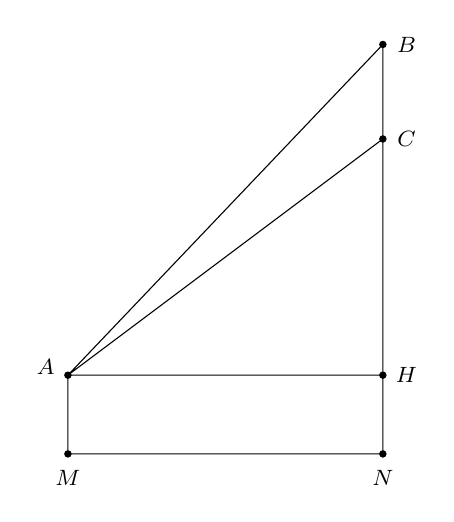
\begin{tikzpicture}[scale=1,font=\footnotesize, line join=round, line cap=round, >=stealth]
			\path 
			(0,0) coordinate (A)
			(4,3) coordinate (C)
			(4,4.2) coordinate (B) 
			(0,-1) coordinate (M) 
			(4,-1) coordinate (N)
			(4,0) coordinate (H) 
			;
			\draw (B)--(A)--(C) (H)--(A)--(M)--(N)--(B);
			\foreach \x/\y in {B/0,C/0,A/160,H/0,M/-90,N/-90}
			\draw[fill=black] (\x) circle (0.04cm) + (\y:0.3cm) node {$\x$};
			\end{tikzpicture}
		}
	}
\end{ex}

\begin{ex}
	\immini{
		Từ một vị trí quan sát $A$, một người nhìn đỉnh $B$ và chân $C$ của nhà cao tầng với các góc tương ứng là $43^{\circ}$ và $16^{\circ}$ so với phương nằm ngang. Biết chiều cao của tòa nhà là $18$ m, tính khoảng cách từ $A$ đến $C$ (làm tròn kết quả đến hàng phần mười).
		\choice
		{$27$ m}
		{$28$ m}
		{\True $29$ m}
		{$31$ m}
	}
	{
		\begin{tikzpicture}[scale=0.8,>=stealth, font=\footnotesize, line join=round, line cap=round]
			\path
			(0,0) coordinate (A)
			(4,3) coordinate (B)
			(4,-1) coordinate (C)
			(4,0) coordinate (H)
			;
			\draw[pattern=bricks,pattern color=brown] (B)--(6,3)--(6,-1)--(4,-1)--(B);
			\foreach \i in {2,3,4,5}
			\draw[fill=white] ({4+1/3},{-1+(2/3)*(\i-1)})--({4+1/3},{-1+(2/3)*(\i-1)+0.5})--({4+2/3},{-1+(2/3)*(\i-1)+0.5})--({4+2/3},{-1+(2/3)*(\i-1)})--cycle
			({5+1/3},{-1+(2/3)*(\i-1)})--({5+1/3},{-1+(2/3)*(\i-1)+0.5})--({5+2/3},{-1+(2/3)*(\i-1)+0.5})--({5+2/3},{-1+(2/3)*(\i-1)})--cycle;
<<<<<<< HEAD
			\draw[dashed](A)--(B) (A)--(C) (A)--(H);
=======
			\draw[dashed](A)--(B)  (A)--(C) (A)--(H);
>>>>>>> fb6a4a45986863e8605634e31e689e31425c42cc
			\draw pic["$43^{\circ}$", draw=black, angle eccentricity=1.4, angle radius=0.9cm]{angle=H--A--B};
			\draw pic["$16^{\circ}$", draw=black,double, angle eccentricity=1.5, angle radius=1.2cm]{angle=C--A--H};
			\foreach \x/\g in {A/180,B/90,C/140,H/145}
			\fill[black] (\x) circle (1pt)+(\g:3mm) node {$\x$};
			\clip (-0.5,{-1-0.25}) rectangle (6.6,-1) ;
			\draw[fill=gray!30] (-0.5,-1)--(6.6,-1)--(6.6,{-1-0.25})--(-0.5,{-1-0.25})--cycle;
			\foreach \i in {1,2,...,35}
			\draw ({-0.5+0.2*(\i)},-1)--($({-0.5+0.2*(\i)},-1)+(-120:0.3)$) ;
		\end{tikzpicture}
	}
	\loigiai{
		Ta có $AH=BH\cot\widehat{BAH}=CH\cot\widehat{CAH}$. \\
		Suy ra
		\begin{align*}
<<<<<<< HEAD
			& (BC-CH)\cot\widehat{BAH}=CH\cot\widehat{CAH} \\
=======
			                & (BC-CH)\cot\widehat{BAH}=CH\cot\widehat{CAH}                         \\
>>>>>>> fb6a4a45986863e8605634e31e689e31425c42cc
			\Leftrightarrow & CH=\dfrac{BC\cot\widehat{BAH}}{\cot\widehat{CAH} +\cot\widehat{BAH}} \\
			\Leftrightarrow & CH=\dfrac{18\cot 43^\circ}{\cot 16^\circ+\cot 43^\circ}.
		\end{align*}
		Khoảng cách từ $A$ đến $C$ là
		\[ AC=\dfrac{CH}{\sin 16^\circ}=\dfrac{18\cot 43^\circ}{(\cot 16^\circ+\cot 43^\circ)\sin 16^\circ}\approx 15{,}4\text{ m.}\]
	}
\end{ex}

\begin{ex}
	Cho tam giác $ABC$ có $a=49{,}4$; $b=26{,}4$; $\widehat{C}=47^{\circ}20'$. Cạnh $c$ gần bằng với số nào sau đây?
	\choice
	{$38$}
	{\True $37$}
	{$39$}
	{$36$}
	\loigiai{
<<<<<<< HEAD
=======
		\begin{eqnarray*}
			&m_a^2=&\dfrac{b^2+c^2}{2}-\dfrac{a^2}{4}. \\
			&m_b^2=&\dfrac{a^2+c^2}{2}-\dfrac{b^2}{4}. \\
			&m_c^2=&\dfrac{a^2+b^2}{2}-\dfrac{c^2}{4}.
		\end{eqnarray*}
		Vậy $S=m_a^2+m_b^2+m_c^2=a^2+b^2+c^2-\dfrac{a^2+b^2+c^2}{4}=\dfrac{3}{4}\cdot(a^2+b^2+c^2)$.}
\end{ex}
\begin{ex}
	Cho tam giác $ABC$ có $a=49{,}4$; $b=26{,}4$; $\widehat{C}=47^{\circ}20'$. Cạnh $c$ gần bằng với số nào sau đây?
	\choice
	{$38$}
	{\True $37$}
	{$39$}
	{$36$}
	\loigiai{
>>>>>>> fb6a4a45986863e8605634e31e689e31425c42cc
		Ta có: $c=\sqrt{a^2+b^2-2ab\cos 47^{\circ}20'} \approx 37$.}
\end{ex}

\TNTF
\begin{ex}%[24-25 giảng K10-K11, Phạm Tuấn]%[0H4H2-1]
Cho tam giác $ABC$. Các khẳng định sau đúng hay sai?
\choiceTF
{\True $\sin A= \sin (B+C)$}
{$R=c\sin C$}
{\True $\cos B = \dfrac{a^2+c^2-b^2}{2bc}$}
{$S=2\sqrt{p(p-a)(p-b)(p-c)}$}
\loigiai{
\begin{itemchoice}
\itemch Vì $\widehat{A}+\widehat{B}+\widehat{C} = 180^\circ$ nên $\sin A= \sin (B+C)$.
\itemch Ta có $R=2c\sin C$.
\itemch Theo định lí cô-sin $\cos B = \dfrac{a^2+c^2-b^2}{2bc}$.
\itemch Theo công thức Heron $S=\sqrt{p(p-a)(p-b)(p-c)}$.
\end{itemchoice}
}
\end{ex}

\begin{ex}%[0-HK1-1-CTST]%[VN-MT-9, Truong Vinh]%[0H4V3-1]
Cho tam giác $ABC$ có $BC=8$, $CA=7$, $AB=5$. Trên cạnh $BC$ lấy điểm $M$ sao cho $BM=5$.
\choiceTF
{$\cos A<0$}
{Chu vi của tam giác $ABC$ bằng $10$}
{Độ dài đường cao xuất phát từ đỉnh $A$ là $h_a=\dfrac{5\sqrt{3}}{4}$}
{\True Độ dài đoạn thẳng $AM$ bằng $5$}
\loigiai{
\begin{center}
\begin{tikzpicture}[scale=0.8, font=\footnotesize, line join=round, line cap=round,>=stealth]
\coordinate (B) at (0,0);
\path
($(B)+(60:5)$) coordinate (A)
($(B)+(0:5)$) coordinate (M)
($(B)+(0:8)$) coordinate (C);
\foreach \x/\g in {A/90,B/180,C/0,M/-90}\fill (\x) circle (1pt) +(\g:0.3) node{\footnotesize$\x$};
\draw (M)--(A)--(B)--(C)--(A);
\end{tikzpicture}
\end{center}
\begin{itemchoice}
\itemch Ta có $\cos A = \dfrac{AB^2+AC^2-BC^2}{2\cdot AB\cdot AC}=\dfrac{5^2+7^2-8^2}{2 \cdot 5 \cdot 7}=\dfrac{1}{7}>0$.
\itemch Chu vi tam giác $ABC$ là $P=AB+AC+BC=5+7+8=20$.
\itemch Nửa chu vi tam giác $ABC$ là $p=\dfrac{P}{2}=10$.\\
$\Rightarrow S_{\triangle ABC} = \sqrt{10\cdot(10-8)\cdot(10-7)\cdot(10-5)}=10\sqrt{3}$.\\
Mà $S_{\triangle ABC}=\dfrac{1}{2}\cdot BC\cdot AH$\\
Vậy ${AH}=\dfrac{2S_{\triangle ABC}}{BC}=\dfrac{20\sqrt{3}}{8}=\dfrac{5\sqrt{3}}{2}$.
\itemch Xét tam giác $ABC$, ta có
\[\cos B= \dfrac{AB^2+BC^2-AC^2}{2\cdot AB\cdot BC} =\dfrac{5^2+8^2-7^2}{2\cdot 5\cdot 8} =\dfrac{1}{2}\Rightarrow \widehat{B}=60^\circ.\]
Xét tam giác $ABM$, ta có $AB=BM=5$; $\widehat{ABM}=60^\circ $.\\
$\Rightarrow \triangle ABM$ là tam giác đều.\\
$\Rightarrow AM=5$.
\end{itemchoice}
}
\end{ex}

\begin{ex}%[0H4V3-2]%[CTST - Lớp 10 - Ôn tập cuối học kì 1 - Đề 2]%[Cao Thành Thái]
Hai người dân đứng cách nhau $30$ m cùng nhìn lên đỉnh của một tòa nhà theo góc nhìn lần lượt là $30^\circ$ và $50^\circ$ (tham khảo hình vẽ).\\
\centerline
{
\begin{tikzpicture}[scale=.5, font=\footnotesize, line join=round, >=stealth]
\coordinate (O) at (0,0);
\def\nhacao{8} %so tang nha cao
\def\dai{.5} %chieu dai 1 khoi
\def\cao{.8} %chieu cao 1 khoi
\newcommand{\xaynha}[2]{
\draw (#1,#2) rectangle (#1+\dai,#2+\cao);
\draw[fill=cyan] (#1,#2) rectangle (#1+\dai,#2+0.25*\cao);
\draw (#1+0.2*\dai,#2+0.25*\cao) rectangle (#1+0.8*\dai,#2+0.9*\cao);
}
\foreach \j in {1,...,\nhacao}{\foreach \i in {0,...,4}{
\xaynha{\i*.6}{\j*\cao}
}
}
\draw[line width=0.2cm,blue] (-0.1,\cao*\nhacao+\cao) -- (5*\dai*1.2,\cao*\nhacao+\cao);
\path (-.1,\cao) coordinate(a) --(5*\dai*1.1,\cao) coordinate(H) ++(90:{8*\cao}) coordinate(C) ++(-50:1) coordinate(c) (C) ++(-30:1) coordinate(c') (intersection of C--c and a--H) coordinate(A) (intersection of C--c' and a--H) coordinate(B);
\draw[very thick] (a) -- (B);
\draw (A)--(C) (B)--(C);
\draw[<->] ([shift={(-90:.2)}]A)--([shift={(-90:.2)}]B) node[midway,below]{$30$ m};
\foreach \d/\g in {A/-135, B/-45, C/90, H/-100}
\fill (\d) circle(1.5pt) node[shift={(\g:.3)}]{$\d$};
\path pic[draw,angle radius=.5cm]{angle=C--B--H} pic[draw,angle radius=.5cm]{angle=C--A--H} pic[draw,angle radius=.6cm]{angle=C--A--H} (B) node[shift={(165:.9)}]{$30^\circ$} (A) node[shift={(155:.9)}]{$50^\circ$};
\end{tikzpicture}
}
\centerline
{
\begin{tikzpicture}[line join=round,font=\large,>=stealth,scale=.5, transform shape]
\tikzset{damlua/.pic={
%define colors
\definecolor{lua}{HTML}{F16414}
\definecolor{luatrong}{HTML}{F5C304}
\definecolor{vienlua}{HTML}{E29D1B}
%Lửa
\fill[lua] (0,1.81) .. controls (-0.7,1.9) and (-2.1,2.3) .. (-0.7,4) .. controls (-1,3.5) and (-1,3.) .. (-0.7,2.9) .. controls (-1.17,3.55) and (0.05,3.9) .. (-0.62,4.67) .. controls (-0.28,4.5) and (-0.15,4.4) .. (-0.14,3.9) .. controls (0.1,4.4) and (-0.75,4.8) .. (-0.1,5.8) .. controls (-0.18,4.8) and (1.15,4.65) .. (0.43,3.57) .. controls (0.6,3.58) and (0.84,4.1) .. (0.72,4.5) .. controls (1.63,3.2) and (0.1,3.15) .. (0.55,2.55) .. controls (0.63,3.2) and (0.9,2.9) .. (1.15,3.65) .. controls (1.5,2.8) and (1.3,1.9) .. cycle;
\fill[vienlua] (0,1.81) .. controls (-0.7,1.9) and (-1.45,2.3) .. (-1.05,3.4) .. controls (-0.9,2.7) and (-0.7,2.82) .. (-0.6,2.83) .. controls (-0.4,2.9) and (-0.3,2.9) .. (-0.2,3.8) .. controls (-0.1,3.4) and (0,3.2) .. (0.1,3) .. controls (0.2,3.1) and (0.35,3.3) .. (0.7,3.58) .. controls (0.34,3.) and (0.39,2.5) .. (0.65,2.45) .. controls (0.7,3.1) and (1,2.9) .. (1.22,3.3) .. controls (1.3,2.7) and (1.3,1.9) .. cycle;
\fill[luatrong] (0,1.81) .. controls (-0.7,1.9) and (-1.45,2.3) .. (-1.1,3.1) .. controls (-0.9,2.7) and (-0.7,2.75) .. (-0.6,2.77) .. controls (-0.4,2.78) and (-0.2,3) .. (-0.2,3.4) .. controls (-0.15,3.3) and (-0.05,3.2) .. (0,2.9) .. controls (0.2,2.9) and (0.35,3.2) .. (0.6,3.45) .. controls (0.3,3.) and (0.35,2.5) .. (0.65,2.41) .. controls (0.9,3) and (1,2.8) .. (1.15,3.1) .. controls (1.3,2.7) and (1.3,1.9) .. cycle;
}}
\tikzset{xecuuhoa/.pic={
\tikzset{banhxe/.pic={
\draw[fill=white](0,0)circle (0.3);
\draw[fill=black!80, even odd rule](0,0) circle (.5) circle (0.3);
\draw[fill](0,0) circle (0.05);
\foreach \i in {1,...,12}{\draw[fill](30*\i:0.15) -- (30*\i:0.25) -- +(90+30*\i:0.05);}
}
}
%-----------Thân xe-----------
\fill[red] (0:0) coordinate(W) -- (90:2) coordinate(B) .. controls ++(90:.8) and ++(200:.8) .. (1,5) coordinate(T) --++(0:4) coordinate(Z) --++(-90:5) coordinate(E) -- cycle;
\draw[fill=red] ([shift={(180:.2)}]E) --++(0:10) coordinate(F) --++(90:3) coordinate(G) ..controls ++(90:.5) and ++(0:.7) .. (13.5,4.3) coordinate(Y) --++(180:8.5) coordinate(I);
\draw (W) -- (B) .. controls ++(90:.8) and ++(200:.8) .. (T) -- (Z) -- (E) -- cycle;
\draw[fill=yellow!60] (5,2.3) coordinate(J) --++(0:9.8) --++(-90:.6) --++(180:9.8) --cycle;
\draw[thin, fill=yellow] (14.78,.3) -- (14.78,.8) .. controls ++(190:.3) and ++(170:.3) .. cycle;
\draw[thin, fill=yellow] (0.02,.5) -- (0.02,1.5) .. controls ++(-10:.5) and ++(10:.5) .. cycle;
\draw[fill=cyan!50] (.6,2.5) --++(80:2) --++(0:1.8) --++(-90:1.98) -- cycle;%kính xe
\draw[fill=cyan!50] (3,2.5) --++(90:2) --++(0:1.5) --++(-90:2) -- cycle;%kính xe
%-----------Gắn bánh xe vào thân xe-----------
\path (2.5,0) pic[scale=2.2]{banhxe} (11.6,0) pic[scale=2.2]{banhxe};
\draw[fill=white] (3.7,0) arc (0:180:1.2) -- ++(180:.2) arc (180:0:1.4) -- cycle;
\draw (3.65,0) arc (0:180:1.15);
\draw[fill=white] (12.8,0) arc (0:180:1.2) -- ++(180:.2) arc (180:0:1.4) -- cycle;
\draw (12.75,0) arc (0:180:1.15);
%-----------Đèn báo hiệu-----------
\draw[fill=red] (2,5) --++(90:.2) .. controls ++(80:.5) and ++(100:.5) .. (3,5.2) --++(-90:.2) -- cycle;
\begin{scope}[shift={(2.5,5.1)}]
\foreach \x in {15,45,...,165}
\draw[red] (\x:.7) -- ++(\x:.3);
\end{scope}
%-----------Thang-----------
\draw[fill=gray] (Y) --++(180:1.5) coordinate(S) --++(90:1.3) coordinate(L) --++(0:.8) --++(-45:.6) -- cycle;
\fill[black!70] ([shift={(-.85,.65)}]Y) circle(.3);
\fill[black] ([shift={(-.85,.65)}]Y) circle(.15);
}}
\coordinate (O) at (0,0);
\def\nhacao{8} %so tang nha cao
\def\dai{.5} %chieu dai 1 khoi
\def\cao{.8} %chieu cao 1 khoi
\newcommand{\xaynha}[2]{
\draw (#1,#2) rectangle (#1+\dai,#2+\cao);
\draw[fill=cyan] (#1,#2) rectangle (#1+\dai,#2+0.25*\cao);
\draw (#1+0.2*\dai,#2+0.25*\cao) rectangle (#1+0.8*\dai,#2+0.9*\cao);
}
\foreach \j in {1,...,\nhacao}{\foreach \i in {0,...,4}{
\xaynha{\i*.6}{\j*\cao}
}}
\draw[line width=0.2cm,blue] (-0.1,\cao*\nhacao+\cao) -- (5*\dai*1.2,\cao*\nhacao+\cao);
\path (-.1,\cao) coordinate(a) --(5*\dai*1.15,\cao) coordinate(H) ++(90:{8*\cao}) coordinate(C) (H) ++(0:{6*\cao}) coordinate(M);
\draw[very thick] (a) -- ([shift={(0:1)}]M);
\path ([shift={(-.4,-1.6)}]C) pic[scale=.6]{damlua} ([shift={(-1.9,.2)}]M) pic[scale=.15]{xecuuhoa};
\draw (M) --++(90:1) coordinate(D) -- (C) -- (H) -- (D) -- ($(C)!(D)!(H)$) coordinate(K);
\draw[<->] ([shift={(0:.4)}]M)--([shift={(0:.4)}]D) node[midway,right]{$1{,}8$ m};
\foreach \d/\g in {M/-90, D/45, C/45, H/-100, K/45}
\fill (\d) circle(1.5pt) node[shift={(\g:.3)}]{$\d$};
\path pic[draw,angle radius=.15cm]{right angle=D--K--H} (D)--(C) node[midway,sloped,above]{$40$ m};
\end{tikzpicture}
}
Các mệnh đề sau đúng hay sai? (Các kết quả làm tròn đến hàng phần chục).
\choiceTF
{Gọi góc nhìn từ đỉnh tòa nhà về hai phía $A$ và $B$ nơi hai người dân đang đứng là góc $\widehat{ACB}$ thì $\widehat{ACB}$ có số đo bằng $30^\circ$}
{\True Khoảng cách từ vị trí người $A$ tới nóc của tòa nhà là $43{,}9$ m}
{Chiều cao của tòa nhà là khoảng $30$ m}
{Vì gặp sự cố nên tầng trên cùng của tòa nhà đang bị cháy. Để cứu hộ đám cháy, một xe cứu hỏa đã tiếp cận dưới chân tòa nhà và chân thang đứng cách mặt đất $1{,}8$ m, chiều dài tối đa của thang xếp là $40$ m. Để tiếp cận được đám cháy thì chân thang của xe cứu hỏa phải đứng cách chân tòa một khoảng xa nhất là $21{,}7$ m}
\loigiai
{
Tam giác $ABC$ có $\widehat{BAC} = 180^\circ-\widehat{CAH} = 180^\circ-50^\circ = 130^\circ$, $\widehat{ABC} = 30^\circ$. Khi đó
\[\widehat{ACB} = 180^\circ-\widehat{BAC} -\widehat{ACB} = 180^\circ - 130^\circ - 30^\circ = 20^\circ.\]
Khoảng cách từ vị trí người $A$ tới nóc của tòa nhà chính là $AC$.\\
Áp dụng định lí Sin trong tam giác $ABC$ ta có
\[\dfrac{AC}{\sin \widehat{ABC}} = \dfrac{AB}{\sin \widehat{ACB}} \Rightarrow AC = \dfrac{AB\sin \widehat{ABC}}{\sin \widehat{ACB}} = \dfrac{30\sin 30^\circ}{\sin 20^\circ} \approx 43{,}9 \text{ (m)}.\]
Do đó, khoảng cách từ vị trí người $A$ tới nóc của tòa nhà là $43{,}9 \text{ m}$.\\
Chiều cao của tòa nhà chính là $CH$.\\
Trong tam giác $CAH$ vuông tại $H$ ta có
\[\sin \widehat{CAH} = \dfrac{CH}{AC} \Rightarrow CH = AC\sin \widehat{CAH} = \dfrac{30\sin 30^\circ}{\sin 20^\circ}\cdot \sin 50^\circ \approx 33{,}6 \text{ (m)}.\]
Do đó, chiều cao của tòa nhà gần bằng $33{,}6 \text{ m}$.\\
Do chân thang cách mặt đất $1{,}8 \text{ m}$ nên $CK=CH-HK \approx 33{,}6-1{,}8=31{,}8 \text{ (m)}$.\\
Khi đó, khoảng cách từ chân thang tới chân tòa nhà xa nhất có thể là
\[KD = \sqrt{CD^2-CK^2} \approx \sqrt{40^2-(31{,}8)^2} \approx 24{,}3 \text{ (m)}.\]
\begin{itemchoice}
\itemch Sai. Do $\widehat{ACB} = 20^\circ$.
\itemch Đúng. Do khoảng cách từ vị trí người $A$ tới nóc của tòa nhà là $AC \approx 43{,}9 \text{ m}$.
\itemch Sai. Do chiều cao của tòa nhà là $CH\approx 33{,}6 \text{ m}$.
\itemch Sai. Do khoảng cách từ chân thang tới chân tòa nhà xa nhất là $KD \approx 24{,}3 \text{ m}$.
\end{itemchoice}
}
\end{ex}

\begin{ex}%[0-TK-HK1-CT-2-2425]%[VN-MT-9-CT-10-11, Võ Nguyên Thạch]%[0H4V3-2]
\immini[thm]{Trên nóc một tòa nhà có một cột ăng-ten cao $5$\,m. Từ một vị trí quan sát $A$ cao $7$\,m so với mặt đất có thể nhìn thấy đỉnh $B$ và chân $C$ của cột ăng-ten, với các góc tương ứng là $50^{\circ}$ và $40^{\circ}$ so với phương nằm ngang (hình vẽ bên) (các kết quả làm tròn đến hàng phần chục).
\choiceTF
{\True Góc $\widehat {ACB}=130^{\circ}$}
{\True $AC \approx 18{,}5$\,(m)}
{$CD \approx 12{,}8$\,(m)}
{Chiều cao của tòa nhà là $19{,}8$\,(m)}
}{
\begin{tikzpicture}[line join=round, line cap=round, >=stealth, scale=1.3, font=\footnotesize]
%		\tikzset{every node/.style={scale=0.8}}
\draw[fill=cyan](0,0) rectangle (1.6,2.6);
\draw[fill=white](0.2,0.2) rectangle (0.6,0.8) (1,0.2) rectangle (1.4,0.8);
\draw[fill=white](0.2,1) rectangle (0.6,1.6) (1,1) rectangle (1.4,1.6);
\draw[fill=white](0.2,1.8) rectangle (0.6,2.4) (1,1.8) rectangle (1.4,2.4);
\coordinate (A) at (3.5,1);
\coordinate (B) at ($(A)+(130:3)$);
\coordinate (C) at ($(A)+(140:2.5)$);
\coordinate (x1) at ($(A)+(180:1.5)$);
\coordinate (x2) at ($(A)+(0:0.5)$);
\draw (A)--(C) (A)--(B) (-0.2,0)--(4,0);
\draw[<->](B)--(C) node[midway, left]{$5$\,m};
\draw[<->](A)--(3.5,0) node[midway, left]{$7$\,m};
\draw (B)--++(20:0.3)--++(160:0.1)--++(210:0.6);
\draw[dashed](x1)--(x2);
\draw pic["$50^\circ$",draw,angle eccentricity=1.2,angle radius=1.6cm]{angle=B--A--x1};
\draw pic["$40^\circ$",draw,double,angle eccentricity=1.4,angle radius=0.8cm]{angle=C--A--x1};
\fill[pattern=north east lines] (-0.2,-0.2) rectangle (4,0);
\foreach \i/\g in {A/90,B/160,C/160}{\fill (\i) circle (1pt) ($(\i)+(\g:7pt)$) node {$\i$};}
\end{tikzpicture}
}
\loigiai{
\begin{center}
\begin{tikzpicture}[line join=round, line cap=round, >=stealth, font=\footnotesize, scale=1]
\def \a{3}
\def \b{3.6}
\def \c{2.5}
\path
(0,0) coordinate (D)
(0:\a) coordinate (A)
(90:\b) coordinate (B)
(90:\c) coordinate (C)   %điều chỉnh độ dài cho đúng tỉ lệ góc
;
%			\coordinate (A) at (3.5,1);
%			\coordinate (B) at ($(A)+(130:3)$);
%			\coordinate (C) at ($(A)+(140:2.5)$);
%			\coordinate (D) at (1.6,1);
\draw (A)--(C) (A)--(B)--(D)--cycle;
\draw pic["$50^\circ$",draw,angle eccentricity=1.2,angle radius=1.6cm]{angle=B--A--D};
\draw pic["$40^\circ$",draw,double,angle eccentricity=1.4,angle radius=0.8cm]{angle=C--A--D};
\foreach \i/\g in {A/90,B/160,C/160,D/180}{\fill (\i) circle (1pt) ($(\i)+(\g:7pt)$) node {$\i$};}
\end{tikzpicture}
\end{center}
\begin{itemchoice}
\itemch {\bf Đúng}.\\
Ta có $\widehat{BAC}=50^{\circ}-40^{\circ}=10^{\circ}$,
$\widehat{ABC}=90^{\circ}-\widehat{BAD}=40^{\circ}$.\\
Suy ra, $\widehat{ACB}=180^{\circ}-\widehat{ABC}-\widehat{BAC}=130^{\circ}$.
\itemch {\bf Đúng}.\\
Áp dụng định lý sin trong tam giác $ABC$ ta có
\[
\dfrac{BC}{\sin A}=\dfrac{AC}{\sin B}\Rightarrow AC=\dfrac{BC \cdot \sin B}{\sin A}=\dfrac{5 \cdot \sin 40^{\circ}}{\sin 10^{\circ}}\approx 18{,}5\,\text{(m).}
\]
\itemch {\bf Sai}.\\
Xét tam giác $ACD$ vuông tại $D$ có $CD=AC \cdot \sin 40^{\circ}\approx 11{,}9$\,(m).
\itemch {\bf Sai}.\\
Chiều cao của tòa nhà là $11{,}9+7=18{,}9$\,(m).
\end{itemchoice}
}
\end{ex}

\TNSA
\begin{ex}%[0-TK-HK1-CT-3-2425]%[VN-MT-9, Chương Ngô Toàn Phúc]%[0H4V1-2]
Cho $\tan x=\dfrac{1}{2}$. Tính giá trị của biểu thức $P=25\left(\sin^4x+\cos^4x\right)$.
\shortans{17}
\loigiai{Ta có
\allowdisplaybreaks
\begin{eqnarray*}
&\sin^4x+\cos^4x&=\left(\sin^2x+\cos^2x\right)^2-2\sin^2x \cdot \cos^2x\\
&&=1-2\sin^2x\cdot\cos^2x\\
&&=1-2\left(1-\cos^2x\right)\cos^2x\\
&&=2\cos^4x-2\cos^2x+1.
\end{eqnarray*}
Từ đó $P=50\left(\cos^4x-\cos^2x\right)+25$.\\
Mặt khác, $\tan^2x+1=\dfrac{1}{\cos^2x} \Rightarrow \cos^2x = \dfrac{1}{1+\tan^2x} = \dfrac{4}{5}$.\\
Dẫn đến $P=50\left(\dfrac{16}{25}-\dfrac{4}{5}\right) + 25 =17$.}
\end{ex}

\begin{ex}%[Mức độ 3]%[Nguyễn Trung Kiên, dự án giảng 10-11, CTGDPT2018]%[0H4V1-2]
Cho $0^\circ <\alpha < 90^\circ$ thỏa mãn $\cos\alpha = \dfrac{5}{6}$. Tính giá trị của biểu thức
\[A=2\sin\left(180^\circ -\alpha\right)\cdot \cot\alpha +\cos\left(180^\circ -\alpha\right)\cdot \tan\alpha \cdot \cot\left(\text{180}^\circ -\alpha\right).\]
\shortans{$2{,}5$}
\loigiai
{Ta có
\begin{align*}
A=&\, 2\sin\left(180^\circ -\alpha\right)\cdot \cot\alpha +\cos\left(180^\circ -\alpha\right)\cdot \tan\alpha \cdot \cot\left(\text{180}^\circ -\alpha\right)\\
=&\, 2\sin\alpha \cdot \cot\alpha +\left(-\cos\alpha\right) \cdot \tan\alpha \cdot \left(-\cot\alpha\right)\\
=&\, 2\sin\alpha \cdot \frac{\cos\alpha }{\sin\alpha }+\cos\alpha \\
=&\, 3\cos\alpha = 3\cdot \dfrac{5}{6} = 2{,}5.
\end{align*}
}
\end{ex}

\begin{ex}%[0H4V2-1]
Cho tam giác $A B C$ có các cạnh $a$, $b$, $c$ thỏa mãn điều kiện $(a+b+c)(a+b-c)=3ab$. Tính số đo của góc $C$ theo đơn vị độ.
\shortans{$60$}
\loigiai{
Trong tam giác $ABC$ ta luôn có $c^2=a^2+b^2-2ab\cos C$.\\
Ta có
\allowdisplaybreaks
\begin{eqnarray*}
(a+b+c)(a+b-c)=3 a b &\Leftrightarrow&(a+b)^2-c^2=3 a b
\\&\Leftrightarrow& c^{2}=(a+b)^2-3 a b   \Leftrightarrow c^2=a^2+b^2-a b \\&\Leftrightarrow& a^2+b^2-2 a b \cdot \cos C=a^2+b^2-a b  \\&\Leftrightarrow&-2 \cos C=-1  \Leftrightarrow \cos C=\dfrac{1}{2} \Leftrightarrow C=60^{\circ}.
\end{eqnarray*}
}
\end{ex}

\begin{ex}%[De-chuan-hoa-so-1]%[Diamond]%[0H4V2-1]
Cho tam giác $ABC$ có $\widehat{A}=60^{\circ} ; \widehat{B}=45^{\circ}$. Tính tỉ số $\dfrac{BC}{AC}$ (làm tròn đến hàng phần trăm).
\shortans[]{$1{,}22$}
\loigiai{
Áp dụng định lí sin ta có
\[
\dfrac{BC}{\sin \widehat{A}} = \dfrac{AC}{\sin \widehat{B}} \Rightarrow \dfrac{B C}{A C} = \dfrac{\sin \widehat{A}}{\sin \widehat{B}} = \dfrac{\dfrac{\sqrt{3}}{2}}{\dfrac{\sqrt{2}}{2}} =  \dfrac{\sqrt{6}}{2}\approx 1{,}22.
\]
}
\end{ex}

\begin{ex}%[0H4H3-2]%[CD-Lớp 10-Ôn tập cuối học kì 1-Đề 5]%[Hoàng Ngọc Lâm]
\immini
{
Trên sườn đồi có một cái cây thẳng đứng (tham khảo hình vẽ) đổ bóng dài $AB=39{,}5$ mét xuống đồi. Biết góc nghiêng của sườn đồi là $\alpha =26^\circ$ so với phương ngang và góc nâng của mặt trời là $\beta =50^\circ$. Tính chiều cao $BC$ của cây (\textit{làm tròn đến hàng đơn vị}).
\shortans[oly]{25}

}{
\begin{tikzpicture}[scale=0.7,font=\footnotesize, line join=round, line cap=round, >=stealth]
\path
(0,0) coordinate (O)
(-3,0) coordinate (A)
(0,4) coordinate (C)
($(A)!1!26:(O)$) coordinate (b)
(intersection of A--b and O--C) coordinate (B);
;

\begin{scope}[shift={(B)}]
\fill[blue!50!yellow] (-.1,0) rectangle (.1,1);
\foreach \x/\y/\z in {1/.6/1.2,.9/.8/1.4,.8/1/1.6,.7/1.2/1.8,.6/1.4/2,.5/1.6/2.2,.4/1.8/2.5}
{
\fill[green!50!black]
(-\x,\y)--(\x,\y)--(0,\z)--cycle;
}

\end{scope}
\draw[dashed] (A)--(O)--(C)--cycle;
\draw[line width=1.2pt,shorten <=-1cm,shorten >=-1cm] (A)--(b);
\draw[dashed,shorten >=-1cm] (A)--(C);
\pic[draw,"$\alpha$", angle eccentricity=1.3,angle radius=0.5cm]{angle=O--A--B};
\pic[draw,below,"$\beta$", angle eccentricity=1.3,angle radius=1cm]{angle=O--A--C};
\draw pic[draw, angle radius=2mm]{right angle=A--O--C};
\foreach \x/\g in {A/-90,C/0,B/-50,O/0} \fill[black] (\x) circle (1pt)+(\g:.3) node {$\x$};
\begin{scope}[shift={($(C)+(1,1.3)$)}]
\fill[orange!30!yellow] (0,0) circle (.5cm);
\foreach \i in {0,30,60,...,360}{
\begin{scope}[rotate=\i]
\draw[orange!30!yellow,line width=1pt] (.7,0)--(1,0);
\end{scope}}
\end{scope}

\end{tikzpicture}
}
\loigiai{
Ta có $\widehat{BAC}=\widehat{OAC}-\widehat{OAB}=24^\circ$ và $\widehat{BCA}=90^\circ-50^\circ=40^\circ$.\\
Áp dụng định lý sin trong $\triangle ABC$, ta có
\allowdisplaybreaks
\begin{eqnarray*}
&&\dfrac{BC}{\sin\widehat{BAC}}=\dfrac{AB}{\sin\widehat{ACB}}\\
&\Rightarrow& BC=\dfrac{AB\cdot\sin\widehat{BAC}}{\sin\widehat{ACB}}\\
&\Rightarrow& BC=\dfrac{39{,}5\cdot\sin 24^\circ}{\sin 40^\circ}\approx 25 ~(\text{m}).
\end{eqnarray*}
}
\end{ex}

\begin{ex}%[Ex-Ôn tập 2025, Hiếu Phan]%[0H4H3-2]
Giả sử ở những giây đầu tiên, máy bay ở \textit{Hình 1} bay theo một đường thẳng tạo với mặt đất một góc $21^\circ$ với vận tốc $240$ km/h. \textit{Hình 2} mô tả mặt đất là một phần mặt phẳng, máy bay bay ở vị trí $I$ đến vị trí $A$. Độ cao $AH$ của máy bay so với mặt đất sau khi máy bay rời khỏi mặt đất $3$ giây là bao nhiêu mét (làm tròn kết quả đến hàng đơn vị)?
\begin{center}

\begin{tikzpicture}[line cap=round,line join=round,>=stealth,font=\footnotesize,scale=.2]
\fill[red!20] (-10,-1.5)--(10,-1.5)--(8,-4)--(-12,-4)--(-10,-1.5);
\begin{scope}[rotate around={21:(0,0)}, scale=0.9] % Xoay hình quanh gốc tọa độ (0,0) góc 20 độ
%%Máy bay
\fill[ball color =cyan!40!gray,rounded corners=0.02](-5.6,3)--++(60:0.8)--++(2:0.55)--++(-90:2)--cycle;
%%Hai cánh
\fill[ball color =cyan!90!gray!40!white](-0.4,1.5)..controls++(75:2)and++(-68:0.75)..(-0.15,4)--++(-5:0.35)..controls++(-50:0.95)and++(106:2)..(1.25,1.5)--cycle;
%Thân
\fill[ball color =cyan!30!gray](-4.85,1)..controls++(-90:0.6) and++(180:0.2)..(-4,0.5)--++(-12:3.3)--++(0:4)..controls++(0:2) and++(-172:1)..(6,0)..controls++(8:1)and++(-90:0.1)..(6.85,0.3)..controls++(90:0.2) and++(-30:1)..(5,1.3)..controls++(90:0.25) and++(0:8)..(-4,1.5)--cycle;
\draw[cyan!40!black](6.85,0.3)coordinate(mui)..controls++(-90:0.5) and++(0:6)..(-2,0.2);
% Cánh phải
\fill[ball color =cyan!90!gray!40!white,rounded corners=0.02](-1.8,0)--++(-5:0.35)--++(-147:4.85)--++(-50:0.7)--++(25.5:6.5)..controls++(-155.5:0.5) and++(-170:0.15)..(1.5,-0.25)..controls++(120:0.5) and++(2:1)..(-1.8,0);
\fill[ball color =cyan!90!gray!40!white,rounded corners=0.02](-6.1,-2.3)--++(-54:0.7)--++(-28:0.7)--++(25.5:.35)--++(-180:.2)--++(135:1.2)--cycle;
%%Thân đuôi
\fill[ball color =cyan!90!gray!40!white,rounded corners=0.02](-6.9,3.6)--++(2:1)..controls++(-35:2) and++(178:2.3)..(-2,1.5)..controls++(-90:0.2) and++(20:1)..(-3.5,1)--++(180:1.2)--cycle;
%%Đuôi
\fill[ball color =cyan!90!gray!40!white,rounded corners=0.02](-6,2.5)--++(0:1.35)--++(-156:2.5)--++(170:0.75)--cycle;
\fill[ball color =cyan!70!gray!40!white,rounded corners=0.02](-1.9,-0.17)--++(90:0.72)--++(181:2.45)--++(-90:0.6)--cycle;
\fill[ball color =cyan!90!gray!10!black,line width=0.02,draw=cyan!30!black,rounded corners=0.005](-1.9,-0.18)arc(-90:270:0.2 and 0.38);
%%Cửa kính
\fill[cyan](5.05,1.3)--++(-25:0.8)..controls++(-140:0.55)and++(10:0.5)..(4.2,0.6)..controls++(180:0.15) and++(182:0.45)..(4.3,1.1)..controls++(2:0.5) and++(-135:0.2)..(5.1,1.3);
\draw[draw=teal,double,distance=0.03](5.05,1.3)++(-26:0.8)..controls++(-140:0.55)and++(10:0.5)..(4.2,0.6)foreach \i in{1,2,...,4}{coordinate[pos=\i/4](B\i)}..controls++(180:0.15) and++(182:0.45)..(4.3,1.1)..controls++(2:0.5) and++(-135:0.2)..(5.1,1.3)foreach \i in{1,2,...,10}{coordinate[pos=\i/10](A\i)}(A2)--(B2)(A6)--(B1);
%Ô cửa trên thân máy bay
\foreach \i in {0,1,...,6}
\fill[ball color=cyan](-0.8+0.5*\i,0.4)arc(-90:270:0.1 and 0.2);
\fill[draw=cyan!10!teal,ball color=cyan!80!gray,rounded corners=0.015](3.2,-0.2)--++(95:0.9)--++(0:0.5)--++(-85:0.9)--cycle;
\begin{scope}[opacity=1]
\fill[ball color=orange](2.5,-0.15)arc(-90:270:0.2 and 0.1);
\fill[ball color=orange!50!red!50!white,rotate around={10:(6,0.25)}](6,0.25)arc(-90:270:0.2 and 0.1);
\end{scope}
\begin{scope}[opacity=0.4]
\fill[ball color=orange](2.5,-0.15)arc(-90:270:0.2 and 0.1);
\fill[ball color=orange!50!red!50!white,rotate around={10:(6,0.25)}](6,0.25)arc(-90:270:0.2 and 0.1);
\end{scope}
\end{scope}
\draw (0,-4) node [below] {\textit{Hình 1}};
\end{tikzpicture}
\begin{tikzpicture}[scale=.6,font=\footnotesize, line join=round, line cap=round, >=stealth]
\coordinate (a) at (0,0);
\coordinate (D) at (8,0);
\coordinate (B) at (-2,-2);
\coordinate (H) at (6,-1);
\coordinate (I) at (1,-1);
\coordinate (C) at ($(B)+(D)-(a)$);
\coordinate (A) at ($(H)+(0,3)$);
\foreach \x/\g in {A/90,H/-100,I/-90} \fill[black](\x) circle (1.5pt) ($(\x)+(\g:3mm)$) node{$\x$};
\draw (H)--(I)--(A) (a)--(B)--(C)--(D)--(a);
\draw[dashed] (H)--(A);
\draw (3,-2.3) node [below] {\textit{Hình 2}};
\end{tikzpicture}
\end{center}
\shortans{$72$}
\loigiai{Máy bay bay với vận tốc là $240$ km/h $=\dfrac{200}{3}$ m/s thì quãng đường đi được sau $3$ giây là \[s=v\cdot t=\dfrac{200}{3}\cdot3=200 \text{ (m)}.\] Suy ra $IA=200$ m.\\
Từ đó ta có độ cao của máy bay so với mặt đất là \[AH=IA\cdot\sin\widehat{AIH}=200\cdot\sin21^\circ\approx 72\text{ (m)}.\]
}
\end{ex}

\begin{ex}%[24-25-Bai-Giang-K10-K11, Tran Quoc]%[0H4V2-2]
\immini[thm]{Một lá cờ hình tam giác cân có độ dài cạnh bên là $90$\,cm và góc ở đỉnh tam giác cân là $35^\circ$. Tính diện tích của lá cờ đó (đơn vị: cm$^2$) với kết quả làm tròn đến hàng đơn vị.}
{
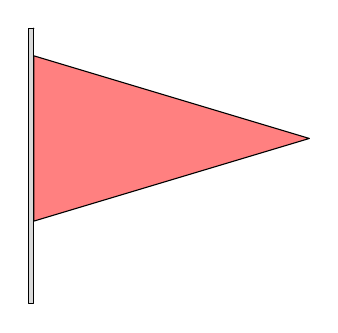
\begin{tikzpicture}[line cap=round,line join=round,scale=0.7]
\path
(0,0) coordinate (C)
(0,3) coordinate (B)
(5,1.5) coordinate (A)
(0,3.5) coordinate (B1)
(0,-1.5) coordinate (C1)
(-0.1,3.5) coordinate (B2)
(-0.1,-1.5) coordinate (C2)
;
\draw[fill=red!50] (A)--(B)--(C)--(A);
\draw[fill=gray!30] (B1)--(B2)--(C2)--(C1)--(B1);
\end{tikzpicture}
}

\shortans{2323}
\loigiai{
\immini{Kí hiệu các điểm $A$, $B$, $C$ như hình bên.\\
Từ giả thiết ta có $AB=AC=90$ cm và $\widehat{A}=35^\circ$. \\
Suy ra $S=\dfrac{1}{2}AB\cdot AC\cdot \sin A=\dfrac{1}{2}\cdot 90
\cdot 90\cdot \sin 35^\circ \approx 2323~\text{cm}^2$. }
{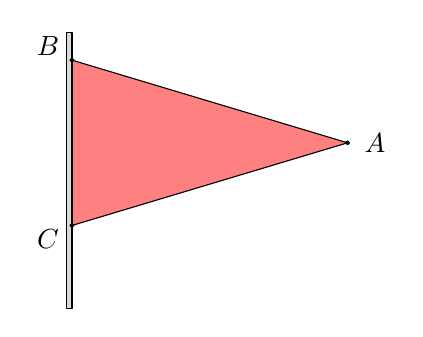
\begin{tikzpicture}[line cap=round,line join=round,scale=0.7]
\path
(0,0) coordinate (C)
(0,3) coordinate (B)
(5,1.5) coordinate (A)
(0,3.5) coordinate (B1)
(0,-1.5) coordinate (C1)
(-0.1,3.5) coordinate (B2)
(-0.1,-1.5) coordinate (C2)
;
\draw[fill=red!50] (A)--(B)--(C)--(A);
\draw[fill=gray!30] (B1)--(B2)--(C2)--(C1)--(B1);
\foreach \d/\g in{A/0,B/150,C/-150}
\draw[fill=black](\d)circle(1pt)node[shift={(\g:0.35)}]{$\d$};
\end{tikzpicture}}
}
\end{ex}

\TL

\begin{ex}
	Chứng minh biểu thức sau độc lập với đối với $x$.
	\[P=\dfrac{\tan^2 x-\cos^2 x}{\sin^2 x}+\dfrac{\cot^2 x-\sin^2 x}{\cos^2 x}.\]
	\loigiai{
		Ta có
		\begin{eqnarray*}
			P&=&\dfrac{\tan^2 x-\cos^2 x}{\sin^2 x}+\dfrac{\cot^2 x-\sin^2 x}{\cos^2 x}\\&=&\dfrac{\tan^2 x}{\sin^2 x}-\dfrac{\cos^2 x}{\sin^2 x}+\dfrac{\cot^2 x}{\cos^2 x}-\dfrac{\sin^2 x}{\cos^2 x}\\
			&=&\tan^2 x(1+\cot^2 x)+\cot^2 x(1+\tan^2 x)-\tan^2 x-\cot^2 x\\&=&\tan^2 x+1+\cot^2 x+1-\tan^2 x-\cot^2 x\\
			&=&2.
		\end{eqnarray*}
		Vậy $P$ không phụ thuộc vào $x$.
	}
\end{ex}
\begin{ex}
	Cho tam giác $ABC$, chứng minh rằng
	$\cos\dfrac{A}{2}=\sqrt{\dfrac{p(p-a)}{b c}}$.
	\loigiai{
		\begin{center}
			\begin{tikzpicture}[scale=1, font=\footnotesize, line join=round, line cap=round, >=stealth]
				\pgfmathsetmacro\a{4/sqrt(3)}
<<<<<<< HEAD
				\path (0,0) coordinate(D) (\a,0) coordinate(A) (5,0) coordinate(C) (30:4) coordinate(B) ($(D)!0.5!(B)$) coordinate (I);
=======
				\path (0,0)  coordinate(D) (\a,0)  coordinate(A) (5,0)  coordinate(C) (30:4) coordinate(B) ($(D)!0.5!(B)$) coordinate (I);
>>>>>>> fb6a4a45986863e8605634e31e689e31425c42cc
				\draw (D)--(B)--(C)--cycle (B)--(A)--(I);
				\foreach \x/\g in {A/-90,B/90,C/-90,D/-90,I/90}\draw[fill=black] (\x) circle (.03) + (\g:.3) node{$\x$};
			\end{tikzpicture}
		\end{center}
		Trên tia đối của tia $AC$ lấy $D$ thỏa $AD=AB=c$ suy ra tam giác $BDA$ cân tại $A$ và $\widehat{BDA}=\dfrac{1}{2} \widehat{BAC}$ (góc ngoài tam giác).
		Áp dụng định lý hàm số cô-sin cho $\triangle ABD$ ta có
		\allowdisplaybreaks
		\begin{eqnarray*}
			BD^{2}&=&AB^{2}+AD^{2}-2AB \cdot AD\cdot\cos\widehat{BAD} \\
			&=&2c^{2}-2c^{2}\cdot\cos\left(180^{\circ}-A\right)\\
			&=&2c^{2}(1+\cos A)=2c^{2}\left(1+\dfrac{b^{2}+c^{2}-a^{2}}{2bc}\right) \\
			&=&\dfrac{c}{b}(a+b+c)(b+c-a)=4c^2\cdot\dfrac{p(p-a)}{bc} \\
<<<<<<< HEAD
			\text {suy ra}\,\, BD&=&2c\sqrt{\dfrac{p(p-a)}{bc}}.
=======
			\text {suy ra}\,\,  BD&=&2c\sqrt{\dfrac{p(p-a)}{bc}}.
>>>>>>> fb6a4a45986863e8605634e31e689e31425c42cc
		\end{eqnarray*}
		Gọi $I$ là trung điểm của $BD$ suy ra $AI \perp BD$.
		Trong tam giác $ADI$ vuông tại $I$, ta có
		$$
			\cos\dfrac{A}{2}=\cos \widehat{ADI}=\dfrac{DI}{AD}=\dfrac{BD}{2c}=\sqrt{\dfrac{p(p-a)}{bc}}.
		$$
		Vậy $\cos \dfrac{A}{2}=\sqrt{\dfrac{p(p-a)}{b c}}$.
	}
<<<<<<< HEAD
\end{ex}

\begin{ex}%[0H4C3-1]
Cho tam giác $ABC$ có thỏa mãn $AC=15$, $AB=10$ và $\sin B=\dfrac{\sin A+\sin C}{\cos A+\cos C}$. Tìm độ dại đoạn $BC$.
% \shortans{30}
\loigiai{
Ta có
\begin{eqnarray*}
&&\sin B=\dfrac{\sin A+\sin C}{\cos A+\cos C}\\
&&\Leftrightarrow \sin B(\cos A+\cos C)=\sin A+\sin C\\
&&\Leftrightarrow \dfrac{b}{2R}\left(\dfrac{b^{2}+c^{2}-a^{2}}{2bc}+\dfrac{a^{2}+b^{2}-c^{2}}{2ab}\right)=\dfrac{a+c}{2R}\\
&&\Leftrightarrow a\left(b^{2}+c^{2}-a^{2}\right)+c\left(a^{2}+b^{2}-c^{2}\right)=2a^{2}c+2c^{2}a\\
&&\Leftrightarrow a^{3}+c^{3}+a^{2}c+ac^{2}-ab^{2}-b^{2}c=0\\
&&\Leftrightarrow (a+c)\left(a^{2}+c^{2}\right)-b^{2}(a+c)=0\\
&&\Leftrightarrow a^{2}+c^{2}=b^{2}.
\end{eqnarray*}
Suy ra tam giác $\triangle ABC$ vuông tại $B$.\\
Từ đó, theo định lý Py-ta-go, ta có $BC=\sqrt{AC^{2}-AB^{2}}=5\sqrt{5}$.
}
=======
>>>>>>> fb6a4a45986863e8605634e31e689e31425c42cc
\end{ex}
\begin{ex}
	Cho tam giác $ABC$ có trọng tâm $G$ và độ dài ba cạnh $AB$, $BC$, $CA$ lần lượt là $15$, $18$, $27$.
	\begin{enumerate}
		\item Tính diện tích và bán kính đường tròn ngoại tiếp tam giác $ABC$.
		\item Tính diện tích tam giác $GBC$.
	\end{enumerate}
	\loigiai
	{
		\begin{enumerate}
			\item %Câu a
<<<<<<< HEAD
			 Nửa chu vi của tam giác $ABC$ là $p=\dfrac{15+18+27}{2}=30$.\\
			 Vậy $S=\sqrt{30\cdot (30-15)\cdot (30-18)\cdot (30-27)}=90\sqrt{2}$.\\
			 Ta có
			 $$S=\dfrac{abc}{4R}\Rightarrow R=\dfrac{abc}{4S}=\dfrac{15\cdot 18 \cdot 27}{4 \cdot 90\sqrt{2}}=\dfrac{81\sqrt{81}}{8}.$$
			\item %Câu b
			 Vì $G$ là trọng tâm của tam giác $ABC$ nên $S_{\triangle GBC}=\dfrac{1}{3}S=30\sqrt{2}$.
=======
			      Nửa chu vi của tam giác $ABC$ là $p=\dfrac{15+18+27}{2}=30$.\\
			      Vậy $S=\sqrt{30\cdot (30-15)\cdot (30-18)\cdot (30-27)}=90\sqrt{2}$.\\
			      Ta có
			      $$S=\dfrac{abc}{4R}\Rightarrow R=\dfrac{abc}{4S}=\dfrac{15\cdot 18 \cdot 27}{4 \cdot 90\sqrt{2}}=\dfrac{81\sqrt{81}}{8}.$$
			\item %Câu b
			      Vì $G$ là trọng tâm của tam giác $ABC$ nên $S_{\triangle GBC}=\dfrac{1}{3}S=30\sqrt{2}$.
>>>>>>> fb6a4a45986863e8605634e31e689e31425c42cc
		\end{enumerate}
	}
\end{ex}

\begin{ex}
	Cho $\cos\alpha=-\dfrac{5}{9}$ và $90^\circ<\alpha<180^\circ$. Tính các giá trị lượng giác còn lại của góc $\alpha$.
	\loigiai{
		$\sin^2\alpha=1-\cos^2\alpha=1-\left(\dfrac59\right)=\dfrac{56}{81}$\\
		$\Rightarrow \sin\alpha=\sqrt{\dfrac{56}{81}}=\dfrac{2\sqrt{14}}{9}$ (vì $\sin\alpha\ge0,\forall \alpha$).\\
		Suy ra $\tan\alpha=\dfrac{\sin\alpha}{\cos\alpha}=-\dfrac{2\sqrt{14}}{5}$ và $\cot\alpha=\dfrac{1}{\tan\alpha}=-\dfrac{5\sqrt{14}}{28}$
	}
\end{ex}
% \begin{ex}
% 	Cho $\heva{&a=\sin x\\&b=\cos x\sin x\\&c=\cos x\cos y}$. Chứng minh rằng $a^2+b^2+c^2=1$.
% 	\loigiai{Ta có:
% 		\begin{align*}
% 		a^2+b^2+c^2 & =\sin^2x+\cos^2x(1-\cos^2y)+\cos^2x\cos^2y \\
% 		&=\sin^2x+\cos^2x-\cos^2x\cos^2y+\cos^2x\cos^2y\\
% 		&=1.
% 		\end{align*}
% 	}
% \end{ex}
\begin{ex}
	Cho tam giác $ABC$, chứng minh rằng	
		 $\cot A+\cot B+\cot C \geq \sqrt{3}$.
	\loigiai{
			Áp dụng định lí côsin và công thức $S=\dfrac{1}{2}bc\sin A$ ta có:\\
			$\cot A=\dfrac{\cos A}{\sin A}=\dfrac{b^{2}+c^{2}-a^{2}}{2 b c \sin A}=\dfrac{b^{2}+c^{2}-a^{2}}{4 S}$.\\
			Tương tự ta có $\cot B=\dfrac{c^{2}+a^{2}-b^{2}}{4 S}, \cot C=\dfrac{a^{2}+b^{2}-c^{2}}{4 S}$\\
			Suy ra $\cot A+\cot B+\cot C=\dfrac{b^{2}+c^{2}-a^{2}}{4 S}+\dfrac{c^{2}+a^{2}-b^{2}}{4 S}+\dfrac{a^{2}+b^{2}-c^{2}}{4 S}=\dfrac{a^{2}+b^{2}+c^{2}}{4 S}$.\\
			Theo bất đẳng thức Cauchy ta có $(p-a) (p-b) (p-c) \leq\left(\dfrac{3 p-a-b-c}{3}\right)^{3}=\left(\dfrac{p}{3}\right)^{3}$.\\
			Mặt khác $S=\sqrt{p(p-a)(p-b)(p-c)} \Rightarrow S \leq \sqrt{p\cdot \dfrac{p^{3}}{27}}=\dfrac{p^{2}}{3 \sqrt{3}}$.\\
			Ta có $p^{2}=\dfrac{\left(a+b+c^{2}\right) }{4} \leq \dfrac{3\left(a^{2}+b^{2}+c^{2}\right) }{4}$ suy ra $S \leq \dfrac{a^{2}+b^{2}+c^{2}}{4 \sqrt{3}}$.\\
			Do đó $\cot A+\cot B+\cot C \geq \dfrac{a^{2}+b^{2}+c^{2}}{4 \cdot \dfrac{a^{2}+b^{2}+c^{2}}{4 \sqrt{3}}}=\sqrt{3}$ .
	}
\end{ex}
\begin{ex}
	Cho tam giác $ABC$ có $AB=6$, $AC=8$ và $\widehat{A}=60^\circ$.
	\begin{enumerate}
		\item Tính diện tích tam giác $ABC$.
		\item Gọi $I$ là tâm đường tròn ngoại tiếp tam giác $ABC$. Tính diện tích tam giác $IBC$.
	\end{enumerate}
	\loigiai
	{
		\immini
		{
			\begin{enumerate}
				\item %Câu a
				Ta có 
				$$S=\dfrac{1}{2}AB\cdot AC\cdot \sin A=\dfrac{1}{2}\cdot 6\cdot 8\cdot \sin60^\circ=12\sqrt{3}.$$
				\item %Câu b
				Ta có $\widehat{BIC}=2\widehat{BAC}=120^\circ$\\
				Ta có
				$$BC=\sqrt{AB^2+AC^2-2AB\cdot AC\cdot \cos A}=\sqrt{6^2+8^2-2\cdot 6\cdot 8\cdot \dfrac{1}{2}}=2\sqrt{13}.$$ 
				Ta có 
				$$S=\dfrac{AB\cdot AC\cdot BC}{4R} \Rightarrow R=\dfrac{AB\cdot BC\cdot CA}{4S}=\dfrac{6\cdot 8\cdot 2\sqrt{13}}{4\cdot 12\sqrt{3}}=\dfrac{2\sqrt{39}}{3}$$
				Từ đó suy ra $IB=IC=R=\dfrac{2\sqrt{39}}{3}$.\\
				Vậy $S_{\triangle IBC}=\dfrac{1}{2}IB\cdot IC\cdot \sin \widehat{BIC}=\dfrac{1}{2}\cdot \dfrac{2\sqrt{39}}{3}\cdot \dfrac{2\sqrt{39}}{3}\cdot \sin 120^\circ\approx 7{,}5$.
			\end{enumerate}	
		}
		{
			\begin{tikzpicture}[scale=0.7, font=\footnotesize, line join=round, line cap=round,>=stealth]
			\def\canhBA{6};\def\canhAC{8};\def\gocBAC{60};
			%Định nghĩa điểm.
			\coordinate (A) at (0,0);
			\coordinate (B) at ($(A)+(\gocBAC:\canhBA)$);
			\coordinate (C) at ($(A)+(0:\canhAC)$);
			%Vẽ tam giác BAC.
			\draw (B)--(A)--(C)--cycle;
			%Hiển thị các điểm.
			\foreach \x/\y in {B/90, A/180, C/0}{\fill (\x) circle(1pt) ($(\x)+(\y:0.3cm)$) node{$\x$};}
			\end{tikzpicture}
		}
	}
\end{ex}

\begin{ex}%[10-11-12EX-HK1-2425]%[Huỳnh Xuân Tín]%[0H4C3-2]
Có hai tàu $A$ và $B$ nằm cùng phía với đường bờ biển (giả sử đường bờ biển là một đường thẳng). Biết tàu $A$, tàu $B$ lần lượt cách đường bờ biển là $3$ hải lí và $6$ hải lí; khoảng cách giữa hai tàu $A$ và $B$ là $5$ hải lí. Người ta muốn xây dựng một trạm nhiên liệu dọc theo đường bờ biển. Hỏi phải đặt trạm nhiên liệu cách tàu $A$ bao nhiêu hải lí để tổng khoảng cách từ trạm nhiên liệu đến hai tàu $A$ và $B$ là ngắn nhất (kết quả làm tròn đến hàng phần chục)?
% \shortans[oly]{$3{,}3$}
\loigiai{\immini{Gọi $H$, $K$ lần lượt là hình chiếu vuông góc của $A$ và $B$ lên đường thẳng $d$ và $D$ là hình chiếu vuông góc của $A$ lên đường thẳng $BK$.\\
Khi đó theo giả thuyết ta có $AH=3$, $BK=6$, $AB=5$. Suy ra $DK=AH=3$.\\
Khi đó $BD=BK-DK=6-3=3$.\\
Tam giác $BDA$ vuông tại $D$ nên $AD=\sqrt{AB^2-BD^2}=\sqrt{5^2-3^2}=4$. Suy ra $HK=AD=4$.\\
Gọi $A'$ đối xứng với $A$ qua đường thẳng $d$.\\
Gọi điểm cần xây dựng một trạm nhiên liệu dọc bờ biển là điểm $M$.\\
Theo tính chất đối xứng thì $MA=MA'$.\\
Khi đó $MA+MB=MA'+MB\ge A'B$. \\
Vậy khi $MA+MB$ nhỏ nhất khi và chỉ khi $A'$, $M$, $B$ thẳng hàng. Khi đó $M$ là giao điểm của $A'B$ với đường thẳng $d$.\\
Suy ra $\dfrac{A'H}{BK}=\dfrac{HM}{MK}=\dfrac{1}{2}\Rightarrow \dfrac{MH}{HK}=\dfrac{1}{3}\Rightarrow MH=\dfrac{4}{3}$.\\
Ta được $AM=\sqrt{AH^2+MH^2}=\sqrt{3^2+\dfrac{16}{9}}\approx 3{,}3$ hải lí.	}{\begin{tikzpicture}[line cap=round,line join=round,scale=0.7,>=stealth,font=\footnotesize]
\coordinate (A) at (1,3);
\coordinate (B) at (5,6);
\coordinate (M) at (7/3,0);
\coordinate (A') at (1,-3);
\coordinate (H) at (1,0);
\coordinate (d1) at (0,0);
\coordinate (K) at (5,0);
\coordinate (D) at (5,3);
\coordinate (d) at (6,0);
\draw[dashed](M)--(A)(A)--(A') (D)--(A)--(B)--(K);
\draw (A')--(B)(d1)--(d)node[above]{$(d)$};
\foreach \x/\g in
{A/90,B/90,A'/-90,M/-50,H/135,K/-90,D/0}
\fill[black](\x) circle (1pt)
($(\x)+(\g:3mm)$) node{$\x$};
\end{tikzpicture}}
Vậy ta cần đặt trạm nhiên liệu cách tàu $A$ một khoản $3{,}3$ hải lí.
}
\end{ex}
\Closesolutionfile{ans}
\Closesolutionfile{ansbook}
% \indapan{10}{ans/ans-KT-301}